% Note that the text in the [] brackets is the one that will
% appear in the table of contents, whilst the text in the {}
% brackets will appear in the main thesis.

%% CHAPTER HEADER /////////////////////////////////////////////////////////////////////////////////////
\chapter[The Time-Domain \acs{sem} Formulation]{The Time-Domain Spectral Element Method Formulation}
\label{ch:sem}
%% CHAPTER INTRODUCTION ///////////////////////////////////////////////////////////////////////////////
The comprehensive formulation of the \ac{sem} based numerical model is presented in this chapter.
It includes shape function definition, numerical integration in the scheme of \ac{gll}, determination of the structural matrices for solid and first-order shear deformation theory elements and electromechanical coupling for the \acp{pzt}.
The non-matching interface was introduced with the novel approach based on the element shape functions.
These components are combined to implement the \ac{sem} for the honeycomb structure with the \ac{fcgm}, which is not found in the literature before.

%% INCLUDE SECTIONS ///////////////////////////////////////////////////////////////////////////////////
%% SECTION HEADER /////////////////////////////////////////////////////////////////////////////////////
\section{The Spectral Element Method}
\label{sec:sem}

%% SECTION CONTENT ////////////////////////////////////////////////////////////////////////////////////

The general concept of the \ac{sem} is based on the idea of the \ac{fem}.
The similarity of both methods lies in the fact that the modeled domain is divided into non-overlapping finite elements, and external forces and arbitrary boundary conditions are imposed in the particular nodes.
The main difference between those methods is a choice of the shape function \( N=N(\xi )\), which is interpolated by a Lagrange polynomial that passes through the element nodes. The nodes are localized on the endpoint of an interval, \(\xi\in[-1,1]\), and the roots of the first derivative of Legendre polynomial P of degree \(p-1\):
\begin{eqnarray}
	(1-\xi^2)P'_{p-1}(\xi)=0.
	\label{eq:nodes}
\end{eqnarray}

The approximation of an integral over the elements is achieved according to \ac{gll} rule at points coinciding with the element nodes, 
and the weights \(w=w(\xi)\) calculated as:
\begin{eqnarray}
	{w(\xi)} = \frac{2}{p(p-1)(P_{p-1}(\xi))^2}.
	\label{eq:weights}
\end{eqnarray}

This approach guarantees a diagonal mass matrix.
The shape functions and the weights for \ac{2d} or \ac{3d} elements are obtained by the Kronecker product of vectors of individual axes, denoted by \(\otimes\) as follows:
\begin{eqnarray}
	N(\xi,\eta) = N(\xi)\otimes N(\eta), & N(\xi,\eta,\zeta) = N(\xi)\otimes N(\eta)\otimes N(\zeta), \nonumber\\
	w(\xi,\eta) = w(\xi)\otimes w(\eta), & w(\xi,\eta,\zeta) = w(\xi)\otimes w(\eta)\otimes w(\zeta).
	\label{eq:3Dshape_weights}
\end{eqnarray}

The elementary equations of motion is defined as:
\begin{eqnarray}
	\label{eq:motion}
	\textbf{M} \ddot{\textbf{d}} + \textbf{D} \dot{\textbf{d}} + \textbf{K} \textbf{d} = \textbf{F}_{ext}
\end{eqnarray}
where \textbf{d} is the displacement vector; \textbf{M}, \textbf{D}, \textbf{K} are structural mass, damping and stiffness matrices, respectively; \textbf{F}$_{ext}$ is the external forces vector; \((\dot{\ })=\frac{\partial}{\partial t}\). Construction of the \textbf{M}, \textbf{D}, \textbf{K} matrices is similar to the classical approach in \ac{fem}.

The convergence of the equation~(\ref{eq:motion}) in the \ac{sem} is already achieved for six nodes per wavelength, while at least fifteen nodes are needed in case of linear elements in classic \ac{fem}~\cite{wee2017simulating}. Moreover, the mass matrix is diagonal when the \ac{gll} approach is used.


%% SECTION HEADER /////////////////////////////////////////////////////////////////////////////////////
\section{2D Spectral Modelling}
\label{sec:2Dmodel}

%% SECTION CONTENT ////////////////////////////////////////////////////////////////////////////////////

According to the first-order shear deformation theory~\cite{reissner1945effect, mindlin1951influence}, the displacement field is expressed as:
\begin{eqnarray}
	\left \{ \begin{array}{c}
		\textbf{u}^e(\xi,\eta) \\
		\textbf{v}^e(\xi,\eta) \\
		\textbf{w}^e(\xi,\eta)
	\end{array} \right\} = 
	\left \{ \begin{array}{c}
		\textbf{u}_0^e(\xi,\eta) + z\boldsymbol{\varphi}_x^e(\xi,\eta)\\
		\textbf{v}_0^e(\xi,\eta) + z\boldsymbol{\varphi}_y^e(\xi,\eta)\\
		\textbf{w}_0^e(\xi,\eta) \\
	\end{array} \right\},
\end{eqnarray}
where \(\textbf{u}_0^e\), \(\textbf{v}_0^e\) and \(\textbf{w}_0^e\) are nodal displacements, \(\boldsymbol{\varphi}_x^e\), \(\boldsymbol{\varphi}_y^e\) are the rotations of the normal to the mid-plane with respect to the axes \textit{x} and \textit{y}, respectively.
\begin{eqnarray}
	\left \{\begin{array}{c}
		\textbf{u}_0^e(\xi,\eta) \\
		\textbf{v}_0^e(\xi,\eta) \\
		\textbf{w}_0^e(\xi,\eta) \\
		\boldsymbol{\varphi}_x^e(\xi,\eta) \\
		\boldsymbol{\varphi}_y^e(\xi,\eta)
	\end{array} \right\}
	= \textbf{N}^e(\xi,\eta)\widehat{\textbf{d}}^e
	= \sum_{n=1}^q\sum_{m=1}^p\textbf{N}_m^e(\xi)\textbf{N}_n^e(\eta)
	\left \{ \begin{array}{c}
		\widehat{\textbf{u}}_0^e \\
		\widehat{\textbf{v}}_0^e \\
		\widehat{\textbf{w}}_0^e \\
		\widehat{\boldsymbol{\varphi}}_x^e \\
		\widehat{\boldsymbol{\varphi}}_y^e
	\end{array} \right \}.
\end{eqnarray}

The nodal bending strain--displacement relations are given in the form:
\begin{eqnarray}
	\boldsymbol{\epsilon}_b^e =
	\textbf{B}_b^e\widehat{\textbf{d}}^e = 
	\left [
	\begin{array}{ccccc}
		\frac{\partial N^e}{\partial x} & 0 & 0 & 0 & 0\\
		0 & \frac{\partial N^e}{\partial y} & 0 & 0 & 0\\
		\frac{\partial N^e}{\partial y} & \frac{\partial N^e}{\partial x} & 0 & 0 & 0\\
		0 & 0 & 0 & -\frac{\partial N^e}{\partial x} & 0\\
		0 & 0 & 0 & 0 & -\frac{\partial N^e}{\partial y}\\
		0 & 0 & 0 & -\frac{\partial N^e}{\partial y} & -\frac{\partial N^e}{\partial x}
	\end{array} \right]
	\left \{ \begin{array}{c}
		\widehat{\textbf{u}}_0^e \\
		\widehat{\textbf{v}}_0^e \\
		\widehat{\textbf{w}}_0^e \\
		\widehat{\boldsymbol{\varphi}}_x^e \\
		\widehat{\boldsymbol{\varphi}}_y^e
	\end{array} \right\}.
\end{eqnarray}

The nodal shear strain--displacement relations are given in the form:
\begin{eqnarray}
	\boldsymbol{\epsilon}_s^e =
	\textbf{B}_s^e\widehat{\textbf{d}}^e = 
	\left [
	\begin{array}{ccccc}
		0 & 0 & \frac{\partial N^e}{\partial y} & -1 & 0\\
		0 & 0 & \frac{\partial N^e}{\partial y} & 0 & -1
	\end{array} \right]
	\left \{ \begin{array}{c}
		\widehat{\textbf{u}}_0^e \\
		\widehat{\textbf{v}}_0^e \\
		\widehat{\textbf{w}}_0^e \\
		\boldsymbol{\varphi}_x^e \\
		\boldsymbol{\varphi}_y^e
	\end{array} \right\}.
\end{eqnarray}
%% SECTION HEADER /////////////////////////////////////////////////////////////////////////////////////
\section{\acs{3d} spectral element}
\label{sec:3Dmodel}

%% SECTION CONTENT ////////////////////////////////////////////////////////////////////////////////////
The displacement vector of the element based on \ac{3d} elasticity of solids is composed of three translational displacements defined as:
\begin{eqnarray}
	\begin{split}
	\left \{ \begin{array}{c}
		\textbf{u}^e(\xi,\eta,\zeta) \\
		\textbf{v}^e(\xi,\eta,\zeta) \\
		\textbf{w}^e(\xi,\eta,\zeta)
	\end{array} \right\}
	& = \textbf{N}^e(\xi,\eta, \zeta)\widehat{\textbf{d}}^e\\
	& = \sum_{l=1}^r\sum_{n=1}^q\sum_{m=1}^p\textbf{N}_m^e(\xi)\textbf{N}_n^e(\eta)\textbf{N}_l^e(\zeta)
	\left \{ \begin{array}{c}
		\widehat{\textbf{u}}^e(\xi_m,\eta_n,\zeta_l) \\
		\widehat{\textbf{v}}^e(\xi_m,\eta_n,\zeta_l) \\
		\widehat{\textbf{w}}^e(\xi_m,\eta_n,\zeta_l)
	\end{array} \right\},
	\label{eq:3D_displ}
	\end{split}
\end{eqnarray}
where \(\widehat{\textbf{u}}^e\), \(\widehat{\textbf{v}}^e\) and 
\(\widehat{\textbf{w}}^e\) are displacements of the element nodes in \(\xi,\eta\) and \(\zeta\) direction.

The nodal strain--displacement relations are given as \cite{kudela20093d}:
\begin{eqnarray}
	\boldsymbol{\varepsilon}^e=\textbf{B}^e\widehat{\textbf{d}}^e=
	\left [
	\begin{array}{ccc}
		\frac{\partial N^e}{\partial x} & 0 & 0\\
		0 & \frac{\partial N^e}{\partial y} & 0\\
		0 & 0 & \frac{\partial N^e}{\partial z}\\
		0 & \frac{\partial N^e}{\partial z} & \frac{\partial N^e}{\partial y}\\
		\frac{\partial N^e}{\partial z} & 0 & \frac{\partial N^e}{\partial x}\\
		\frac{\partial N^e}{\partial y} & \frac{\partial N^e}{\partial x} & 0
	\end{array} \right]
	\left \{ \begin{array}{c}
		\widehat{\textbf{u}}^e \\
		\widehat{\textbf{v}}^e \\
		\widehat{\textbf{w}}^e
	\end{array} \right\}.
\end{eqnarray}
The formulae of the structural matrices for \ac{3d} elements are:
\begin{eqnarray}
	\textbf{M}_{dd}^e & = & \int_{V^e}\textbf{N}^{\mathrm{T}}\rho \textbf{N} \diff V^e,\\
	\textbf{K}_{dd}^e & = & \int_{V^e}{\textbf{B}_d^e}^{\mathrm{T}}\textbf{c}\textbf{B}_d^e \diff V^e,
\end{eqnarray}
\nomtypeR[Ve]{$V^e$}{Element volume}{-}{\unit{\cubic\meter}}%
where \textbf{c} is the elasticity tensor, \(\rho\) is mass density, and \(V_e\) is the element volume.
%% SECTION HEADER /////////////////////////////////////////////////////////////////////////////////////
\section{Piezoelectric Transducers Modelling}
\label{sec:PZTmodel}

%% SECTION CONTENT ////////////////////////////////////////////////////////////////////////////////////
The electromechanical coupling is governed by the linear constitutive equation of piezoelectric material according to~\cite{giurgiutiu2009micromechatronics, rekatsinas2017cubic}, and this is defined as:
\begin{eqnarray}
	\left [ 
	\begin {array}{c}
	\boldsymbol{\sigma}\\
	\textbf{D}
\end{array}\right ]=
\left [ 
\begin{array}{cc}
	\textbf{c}^E & -\textbf{e}^T \\
	\textbf{e} & \epsilon^S 
\end{array} \right ]
\left[ 
\begin{array}{c}
	\textbf{S}\\
	\textbf{E} 
\end{array} \right ],
\label{eq:elecmechcoupling}
\end{eqnarray}
where \(\boldsymbol{\sigma}\) and \(\textbf{S}\) are the stress and strain components, respectively, \(\textbf{c}^E\) is the stiffness coefficient matrix measured at zero electric field, \textbf{e} is the piezoelectric coupling tensor,  \(\boldsymbol{\epsilon}^S\) is the electric permittivity, and \textbf{E} and \textbf{D} are the electric field and electric displacement measured at zero strain.
The superscript T denotes a transpose matrix.
The electric field is defined as:
\begin{eqnarray}
\textbf{E}^e=-\textbf{B}_\phi^e \widehat{\boldsymbol{\phi}}^e = \left[ \begin{array}{c}
	\frac{\partial N^e}{\partial \xi}\\
	\frac{\partial N^e}{\partial \eta}\\
	\frac{\partial N^e}{\partial \zeta}
\end{array} \right] \widehat{\boldsymbol{\phi}}^e,
\end{eqnarray}
where \(\widehat{\boldsymbol{\phi}}^e\) is a nodal voltage of the transducer. The \ac{sem} formulation of the governing equation (\ref{eq:elecmechcoupling}) is defined as:
\begin{eqnarray}
	\left [\begin{array}{cc}
		\textbf{M}_{dd} & \textbf{0}\\
		\textbf{0} & \textbf{0}
	\end{array}\right]
	\left \{\begin{array}{c}
		\widehat{\ddot{\textbf{d}}} \\
		\textbf{0}
	\end{array}\right \} +
	\left [\begin{array}{cc}
		\textbf{K}_{dd} & \textbf{K}_{d \phi}\\
		\textbf{K}_{d \phi}^T & \textbf{K}_{\phi \phi}
	\end{array}\right]
	\left \{\begin{array}{c}
		\widehat{\textbf{d}} \\
		\widehat{\boldsymbol{\phi}}
	\end{array}\right \}  = 
	\left \{\begin{array}{c}
		\textbf{0}\\
		\widehat{\textbf{Q}}
	\end{array}\right \},
	\label{eq:pzt_sem}
\end{eqnarray}
where \(widehat{\textbf{Q}}\) is the nodal charge vector.
The mass and stiffness matrices are defined according to \ac{3d} model from section \ref{sec:3Dmodel}.
The piezoelectric coupling matrix \(\textbf{K}_{\phi \phi}^e\) and the dielectric permittivity matrix \(\textbf{K}_{d \phi}^e\) are defined as:
\begin{eqnarray}
	\textbf{K}_{d\phi}^e & = & \int_{V_e}{\textbf{B}_d^e}^T\textbf{e}^T \textbf{B}_{\phi}^e \diff V_e,\\
	\textbf{K}_{\phi \phi}^e & = & -\int_{V_e}{\textbf{B}_{\phi}^e}^T 
	{\textbf{\(\epsilon\)}^S}^T \textbf{B}_{\phi}^e \diff V_e.
\end{eqnarray}

If a vector \(\textbf{b}\) contains list of consecutive boundary nodes (electrodes) and a vector \(\textbf{a}\) contains lists of consecutive active nodes (remains nodes) of the \ac{pzt}, the electrical potential vector and the charge vector can be rewritten as:
\begin{eqnarray}
	\widehat{\boldsymbol{\phi}} & = & \left \{\begin{array}{cc}
		\widehat{\boldsymbol{\phi}}(\textbf{b}) &
		\widehat{\boldsymbol{\phi}}(\textbf{a})
	\end{array}\right \}^T,\\
	\widehat{\textbf{Q}} & = & \left \{\begin{array}{cc}
		\widehat{\textbf{Q}}(\textbf{b}) & \textbf{0}
	\end{array}\right \}^T.
	\label{eq:phi_Q}
\end{eqnarray}
Then, piezoelectric part of Equation~(\ref{eq:pzt_sem}) is expressed as:
\begin{eqnarray}
	\left [\begin{array}{cc}
		\textbf{K}_{d \phi}(:,\textbf{b}) &
		\textbf{K}_{d \phi}(:,\textbf{a})
	\end{array}\right]^T
	\widehat{\textbf{d}} +
	\left [\begin{array}{cc}
		\textbf{K}_{\phi \phi}(\textbf{b},\textbf{b}) & \textbf{K}_{\phi \phi}(\textbf{b},\textbf{a})\\
		\textbf{K}_{\phi \phi}(\textbf{a},\textbf{b}) & \textbf{K}_{\phi \phi}(\textbf{a},\textbf{a})
	\end{array}\right]
	\left \{\begin{array}{c}
		\widehat{\boldsymbol{\phi}}(\textbf{b}) \\
		\widehat{\boldsymbol{\phi}}(\textbf{a})
	\end{array}\right \} = 
	\left \{\begin{array}{c}
		\widehat{\textbf{Q}}(\textbf{b}) \\
		\textbf{0}
	\end{array}\right \},
	\label{eq:pztboundary}
\end{eqnarray}
where the notation \(\textbf{K}(\textbf{r},\textbf{c})\) uses vectors \(\textbf{r}\) and \(\textbf{c}\) to extract rows and columns from the matrix \(\textbf{K}\), respectively, and \((:)\) means all rows or columns of \(\textbf{K}\).
The electrical potential of the free nodes can be extracted from Equation~(\ref{eq:pztboundary}):
\begin{eqnarray}
	\widehat{\boldsymbol{\phi}}(\textbf{a}) = -\textbf{K}_{\phi\phi}^{-1}(\textbf{a},\textbf{a})\left[\textbf{K}_{\phi d}(\textbf{a},:) \widehat{\textbf{d}} + \textbf{K}_{\phi\phi}(\textbf{a},\textbf{b})\widehat{\boldsymbol{\phi}}(\textbf{b}) \right].
	\label{eq:freePotetial}
\end{eqnarray}
If the \ac{pzt} acts as an actuator, the electrical potential of the electrode nodes has the values of the applied signal.
As one of the electrodes is grounded, the potential is zero.
Therefore, the potential vector can be written as:
\begin{eqnarray}
	\widehat{\boldsymbol{\phi}}(\textbf{b}) = \left \{\begin{array}{cc}
		\widehat{\boldsymbol{\phi}}(\textbf{b}_v) &
		\widehat{\boldsymbol{\phi}}(\textbf{b}_g)
	\end{array}\right \}^T=\left \{\begin{array}{cc}
	\textbf{V}(t) & \textbf{0}
	\end{array}\right \}^T,
	\label{eq:phi_V}
\end{eqnarray}
where \(\textbf{b}_v\) is a list of nodes of the applied electrode and \(\textbf{b}_g\) is a list of nodes of the grounded electrode.
Substituting Equation (\ref{eq:phi_V}) into Equations (\ref{eq:freePotetial}) and (\ref{eq:pztboundary}) induced stiffness of the actuator is obtained:
\begin{eqnarray}
	\textbf{K}_{a}=-\textbf{K}_{d\phi}(:,\textbf{a})\,\textbf{K}_{\phi \phi}^{-1}(\textbf{a},\textbf{a})\,\textbf{K}_{\phi \phi} (\textbf{a},\textbf{b}).
\end{eqnarray}
Hence, the equivalent mechanical force vector of the applied voltage of the piezoelectric actuator equals:
\begin{eqnarray}
	\widehat{\textbf{f}}_{act}=-\textbf{K}_{a}\,\widehat{\boldsymbol{\phi}}(\textbf{b}).
	\label{eq:f_act}
\end{eqnarray}

In the case of the open circuit sensor one electrode is grounded so the electric potential of the free nodes becomes as:
\begin{eqnarray}
	\widehat{\boldsymbol{\phi}}(\textbf{a}) = -\textbf{K}_{\phi\phi}^{-1}(\textbf{a},\textbf{a})\,\textbf{K}_{\phi d}(\textbf{a},:)\,\widehat{\textbf{d}}.
	\label{eq:sensorPotetial}
\end{eqnarray}
The induced stiffness of the sensor can be written as:
\begin{eqnarray} \textbf{K}_s=\textbf{K}_{d \phi}(:,\textbf{a})\,\textbf{K}_{\phi \phi}^{-1} (\textbf{a},\textbf{a})\,\textbf{K}_{\phi d}(\textbf{a},:).
\end{eqnarray}
To obtain the sensor response nodal electric potential must be integrated over the electrode surface as follow:
\begin{eqnarray}
	\boldsymbol{\phi}(t) = \int_{\Omega_s}\widehat{\phi} \diff\Omega_s.
	\label{eq:sensorResponse}
\end{eqnarray}
%% SECTION HEADER /////////////////////////////////////////////////////////////////////////////////////
\section{Structural damping}
\label{sec:damping}

%% SECTION CONTENT ////////////////////////////////////////////////////////////////////////////////////
Propagating waves in the structure attenuate due to many factors, including geometric spreading, material damping, and dissipation into the adjacent domain.
This study adopted the Rayleigh damping model for the \ac{cfrp} skin and adhesive layer, while the damping for the aluminium core and \ac{pzt} was neglected.
Rayleigh damping model is defined as \cite{wandowski2017guided}:
\begin{eqnarray}
	\textbf{D}_{dd}^e = \alpha_M \textbf{M}_{dd}^e + \beta_K \textbf{K}_{dd}^e,
	\label{eq:damping}
\end{eqnarray}
where \(\alpha_M\) and \(\beta_K\) are the mass- and stiffness- proportionality coefficients.
In presented model, \(\beta_K\) was assumed equal to zero to ensure that matrix \(\textbf{D}_{dd}\) remains diagonal \cite{schulte2011simulation, wandowski2017guided}.
This assumption gives a good approximation when considering a single mode and a specific frequency. 
Ramadas showed slight differences in Lamb wave attenuation by analysing three models, i.e. mass-, stiffness-proportional and the sum of both \cite{ramadas2011modelling}.
However, the mass-proportional model is computationally incomparable to the other models due to the diagonal damping matrix.
%% SECTION HEADER /////////////////////////////////////////////////////////////////////////////////////
\section{Displacements coupling at the interface of substructures}
\label{sec:interface}

%% SECTION CONTENT ////////////////////////////////////////////////////////////////////////////////////

The present model of the sandwich panel consists of \ac{2d} and \ac{3d} elements. 
Moreover, there are non-matching grids between two adjacent substructures. 
These involve connecting them by imposing the compatibility of the displacements at the interface, see Fig.~\ref{fig:interface}.
This type of connection is implemented through the interface elements based on Lagrange multipliers, which are interpreted as forces responsible for determining the appropriate displacements of nodes.
The coupling can be expressed as:
\begin{eqnarray}
	\left\{\begin{array}{c}
		\textbf{u}\\
		\textbf{v}\\
		\textbf{w}
	\end{array}\right\}_{s_{i1}}^{\Gamma^i}-
	\left\{\begin{array}{c}
		\textbf{u}\\
		\textbf{v}\\
		\textbf{w}
	\end{array}\right\}_{s_{i2}}^{\Gamma^i}=
	\left\{\begin{array}{c}
		\textbf{0}\\
		\textbf{0}\\
		\textbf{0}
	\end{array}\right\},
	\label{eq:coupling}
\end{eqnarray}
\begin{figure}
	\begin{center}
		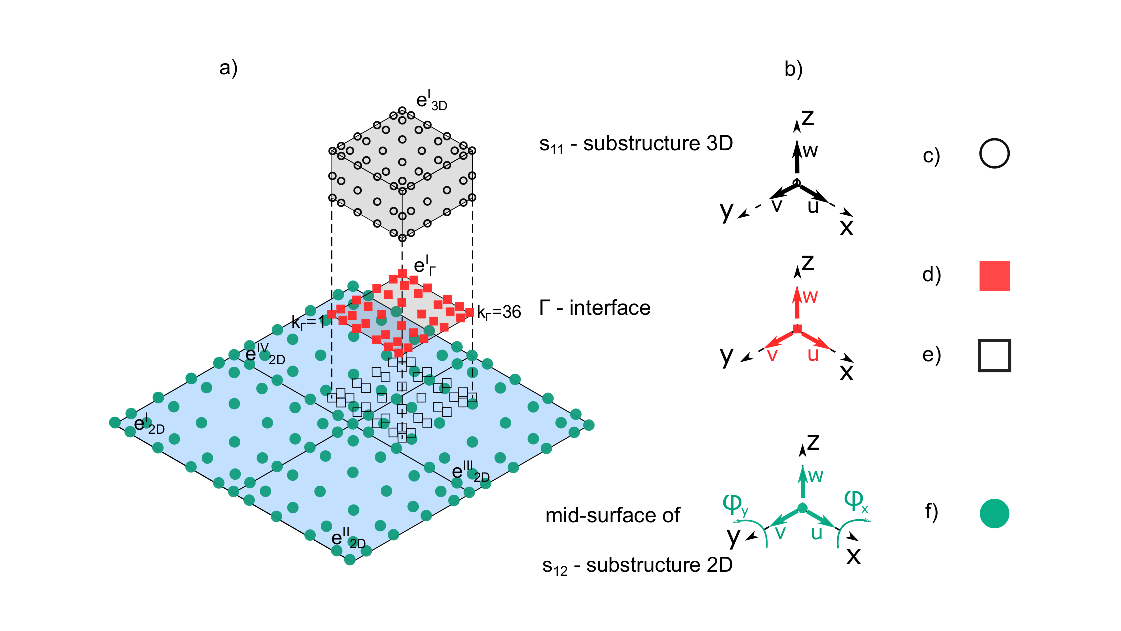
\includegraphics[width=0.95\textwidth]{Chapter_4/interface_2D3D}
	\end{center}
	\caption{Non-matching interface setup: a) interface coupling, b) degrees-of-freedom of the interface and the substructures.}
	\label{fig:interface}
\end{figure}
where \(s_{i1}\) and \(s_{i2}\) are substructures connected by the interface \(\Gamma^i\). For the whole structure, the Eq.~(\ref{eq:coupling}) can be written in the matrix form:
\begin{eqnarray}
	\textbf{G}\textbf{d}=\textbf{0},
	\label{eq:cond_disp}
\end{eqnarray}
where \textbf{G} is the coupling matrix which contains the equations to interpolate the substructures displacements at the interfaces, and \(\textbf{d}\) is a global displacement field for \(nS\) number of substructures, composed as:
\begin{eqnarray}
	\textbf{d} = \left\{\begin{array}{cccc}
		\textbf{d}_1, & \textbf{d}_2, &\ldots, & \textbf{d}_{nS}
	\end{array}\right\}^T.
	\label{eq:displacements}
\end{eqnarray}

General formulation of the matrix \textbf{G} is presented in Algorithm \ref{alg:G_matrix}.

\begin{algorithm}[H]
	\SetAlgoLined
	\KwResult{coupling matrix \textbf{G}}
	\For{i = 1 \KwTo 2}{
		create \(n^{\Gamma}\times n^{s_i}\) null matrix 
		\(\mathbf{G}_i\),\\
		\For{j = 1 \KwTo \(n^{\Gamma}\)} {
			find \(ownerElement^j_i\) in the structure \(s_i\) 
			containing interface node \(j\) with global coordinates vector: 
			\(X_p=(x^j_p,y^j_p)\)\;
			assign vector \(X_e=(x_e,y_e)\) of coordinates of all nodes in 
			\(ownerElement^j_i\)\;
			assign initial coordinates 
			\(X_{\kappa}=(x^j_{\kappa},y^j_{\kappa})\) to the nearest node in
			\(ownerElement^j_i\) to node \(j\)\;
			transform global coordinates \(X_{\kappa}\) to a local coordinate system \(\xi_{\kappa}=\xi(X_{\kappa});\quad 
			\eta_{\kappa}=\eta(X_{\kappa})\)\;
			\While{\(\left|X_p-X_{\kappa}\right|>tol\)}{
				\(\xi_{\kappa+1}=\xi_{\kappa}+(\mathcal{J}_{\kappa})^{1,1}_{\mathrm{inv}}.*(x^j_p-x_{\kappa}^j)
				+(\mathcal{J}_{\kappa})^{1,2}_{\mathrm{inv}}.*(y^j_p-y_{\kappa}^j)\)\;
				\(\eta_{\kappa+1}=\eta_{\kappa}+(\mathcal{J}_{\kappa})^{2,1}_{\mathrm{inv}}.*(x^j_p-x_{\kappa}^j)
				+(\mathcal{J}_{\kappa})^{2,2}_{\mathrm{inv}}.*(y^j_p-y_{\kappa}^j)\)\;
				\(X_{\kappa}=N_{\kappa+1}X_e\)\;
			}
			\(\mathbf{G}_i(j,n^{X_e})=N_{\kappa+1}\)\;
		}
		\uIf{\(s_i\) is \(\mathrm{3D}\)} {
			\(\mathbf{G}_i=\left[\begin{array}{ccc}
				\mathbf{G}_i & \mathbf{0} & \mathbf{0}\\
				\mathbf{0} & \mathbf{G}_i & \mathbf{0}\\
				\mathbf{0} & \mathbf{0} & \mathbf{G}_i
			\end{array} \right]
			\)\;
		}
		\ElseIf{\(s_i\) is \(\mathrm{2D}\)} {
			\(\mathbf{G}_i=\left[\begin{array}{ccccc}
				\mathbf{G}_i & \mathbf{0} & \mathbf{0} & 
				\frac{h_i}{2}\mathbf{G}_i & \mathbf{0}\\
				\mathbf{0} & \mathbf{G}_i & \mathbf{0} & \mathbf{0} & 
				\frac{h_i}{2}\mathbf{G}_i\\
				\mathbf{0} & \mathbf{0} & \mathbf{G}_i & \mathbf{0} & 
				\mathbf{0}
			\end{array} \right]\)\;
		}
	}
	\(\mathbf{G}=\left[\begin{array}{cc}
		\mathbf{G}_1 & \mathbf{G}_2
	\end{array} \right]\)
	\caption{Interface coupling matrix formulation}
	\label{alg:G_matrix}
\end{algorithm}
where \(s_i\) is one of the coupled structures, \(n^{\Gamma}\) and \(n^{s_i}\) are node numbers of the interface and node numbers of the structure \(s_i\), respectively; \(\left(\mathcal{J}_{\kappa}\right)_{\mathrm{inv}}\) is the inverse Jacobian matrix evaluated at \((\xi_{\kappa},\eta_{\kappa})\) and \(N_{\kappa+1}\) is the shape function evaluated at \((\xi_{\kappa+1},\eta_{\kappa+1})\), \(n^{X_e}\) is the vector of global order numbers of all nodes in the \(ownerElement^j_i\), \(h_i\) is a thickness of the structure \(s_i\) and \(tol\) is a termination criterion for iterations.

The main task of the algorithm is to calculate shape functions for each adjacent substructure at the points \(X_p=(x_p^k,y_p^k)\), which are projections of the interface nodes onto these substructures.
The shape function can be calculated after finding an owner element and local coordinates of the points.
Owner element is a spectral element in the domain of the substructure \(s_{ij}\) which contains interface node, for example, interface node \(k_\Gamma=36\) (see~Fig.~\ref{fig:interface}a)) is located in the element \(e^{I}_{3\mathrm{D}}\) and \(e^{III}_{2\mathrm{D}}\) for the substructures \(s_{11}\) and \(s_{12}\), respectively.
It can be found within two ways: using Matlab's built-in function \verb+inpolygon+ or more efficient procedure proposed by Silva et al. \cite{silva2009exact} which was used in the current implementation.
In this procedure, an initial approximation is first performed by rejecting all external points outside the rectangular region bounded by the points \(\mathrm{P_{min}}\) and \(\mathrm{P_{max}}\) as shown in Fig. \ref{fig:b_b_test}(\textbf{a}).
If \(\mathrm{X_p}\) is inside the element, then the vectors \(V_1\) and \(V_2\) have the same direction.
\(V_1\) and \(V_2\) are defined as:
\begin{eqnarray}
	\vec{V}_1 & = & \vec{v}_-\times \vec{v},\\
	\vec{V}_2 & = & \vec{v}\times \vec{v}_+.
\label{eq:v_vectors}
\end{eqnarray}
The vectors \(\vec{v}\), \(\vec{v_-}\) and \(\vec{v_+}\) are pictured in Fig. \ref{fig:b_b_test}(\textbf{b}). \(V_1\) and \(V_2\) will have the same direction if the inequality is satisfied for each element vertex \(i\):
\begin{eqnarray}
		\vec{V}_1 \cdot \vec{V}_2 \geq0.
	\label{eq:dot_prod}
\end{eqnarray}
Then, the transformation from global to local coordinates is realised by the iterative method presented in the work of Li et al.~\cite{li2014efficient} (see also \verb+while-loop+ in Alg. \ref{alg:G_matrix}).
\begin{figure}[H]
	\begin{center}
		\includegraphics[width=0.95\textwidth]{Chapter_4/b_b_test}
	\end{center}
	\caption{Owner element for Xp interface node (\textbf{a}) boundary test, (\textbf{b}) cross-product test}
	\label{fig:b_b_test}
\end{figure}
While the cross-product test is exact for elements with linear edges, the approximation of the boundary test is used for second order elements, and then \(\xi_{\kappa}\) and \(\eta_{\kappa}\) must satisfy the condition \(-1\leq \xi_{\kappa},\eta_{\kappa} \leq 1\).
The computational effectiveness of Algorithm~\ref{alg:G_matrix} can be easily improved if certain precautions are taken.
Firstly, the mesh of the interface has to be based on the mesh from one of the substructures \(s_{i}\), which may be referred to as a slave.
So, shape functions evaluated at (\(\xi\), \(\eta\)) may take only zero and one values.
Moreover, the code was vectorised rather than using a for-loop form, provided that the required matrix of size \(4n^e\times n^{\Gamma}\), where \(n^e\) is the number of elements of the structure \(s_i\) elements, does not exceed the operating memory.
%% SECTION HEADER /////////////////////////////////////////////////////////////////////////////////////
\section{Transformation of the core elements}
\label{sec:transformation}

%% SECTION CONTENT ////////////////////////////////////////////////////////////////////////////////////
All core elements are rotated relative to both skins, and thus it is necessary to transform the degrees of freedom from the local coordinate system of the core to the global coordinate system.
For this purpose, an additional sixth \ac{dof} was incorporated, i.e., rotation with respect to the \textit{z}-axis:
\begin{eqnarray}
	\widehat{\textbf{d}}^e_g = \left \{\begin{array}{cccccc}
		\widehat{\textbf{u}}^e & \widehat{\textbf{v}}^e &
		\widehat{\textbf{w}}^e & \widehat{\boldsymbol{\varphi}}_x^e &
		\widehat{\boldsymbol{\varphi}}_y^e & \widehat{\boldsymbol{\varphi}}_z^e
	\end{array}\right \}^{\mathrm{T}}_g.
	\label{eq:d6}
\end{eqnarray}

First, the displacement vector was transformed from the global to local coordinate system by the direction cosines as follows
\begin{eqnarray}
	\widehat{\textbf{d}}^e_l = \left \{\begin{array}{c}
		\widehat{\textbf{u}}^e \\ \widehat{\textbf{v}}^e \\
		\widehat{\textbf{w}}^e \\ \widehat{\boldsymbol{\varphi}}_x^e \\
		\widehat{\boldsymbol{\varphi}}_y^e
	\end{array}\right \}_l = 
	\left [\begin{array}{ccccc}
		\mathcal{V}^e_1, & \mathcal{V}^e_2, & \mathcal{V}^e_3, & \textbf{0} & \textbf{0} \\
		\textbf{0} & \textbf{0} & \textbf{0} & \mathcal{V}^e_1, & \mathcal{V}^e_2
	\end{array}\right ]^{\mathrm{T}}
	\left \{\begin{array}{c}
		\widehat{\textbf{u}}^e \\ \widehat{\textbf{v}}^e \\
		\widehat{\textbf{w}}^e \\ \widehat{\boldsymbol{\varphi}}_x^e \\
		\widehat{\boldsymbol{\varphi}}_y^e\\
		\widehat{\boldsymbol{\varphi}}_z^e
	\end{array}\right \}_g,
	\label{eq:d_local}
\end{eqnarray}
\nomtypeD[vector_cos]{\(\mathcal{V}^e_1,\,\mathcal{V}^e_2,\,\mathcal{V}^e_3\)}{Direction cosines}{}%
where \(g\) and \(l\) mean global and local coordinate system, respectively, \(\mathcal{V}^e_1\),\(\mathcal{V}^e_2\) and \(\mathcal{V}^e_3\) are direction cosines of the core element.
Then, internal forces were calculated according to guideline from Section \ref{sec:gpu} and transformed to a global coordinate system by the direction cosines as
\begin{eqnarray}
	\left\{\textbf{F}_{int}\right\}^e_g =
	\left [\begin{array}{ccccc}
		\mathcal{V}^e_1, & \mathcal{V}^e_2, & \mathcal{V}^e_3, & \textbf{0} & \textbf{0} \\
		\textbf{0} & \textbf{0} & \textbf{0} & \mathcal{V}^e_1, & \mathcal{V}^e_2
	\end{array}\right ]
	\left \{\begin{array}{c}
		\textbf{F}^1_{int} \\
		\textbf{F}^2_{int} \\
		\textbf{F}^3_{int} \\
		\textbf{F}^4_{int} \\
		\textbf{F}^5_{int} \\
	\end{array}\right \}_l^e.
	\label{eq:f_global}
\end{eqnarray}

Additionally, a part of the mass matrix accounted for rotational inertia was transformed, and, in contrast to the vector of internal forces, it had to be done only once in pre-processing as follows:

\begin{eqnarray}
	\textbf{J}_g=\left [ 
	\begin{array}{ccc}
		\left (\textbf{J}\right)^{1,1}_g & \left (\textbf{J}\right )^{1,2}_g & \left (\textbf{J}\right )^{1,3}_g\\
		& \left (\textbf{J}\right )^{2,2}_g & \left (\textbf{J}\right )^{2,3}_g\\
		Sym. &  & \left (\textbf{J}\right )^{3,3}_g\\
	\end{array}
	\right ]
	=\left[\begin{array}{ccc}
		\mathcal{V}_1, \mathcal{V}_2, \mathcal{V}_3 \end{array}\right ]^{\mathrm{T}}
	\,\textbf{J}_l\,
	\left[\begin{array}{ccc}
		\mathcal{V}_1, \mathcal{V}_2, \mathcal{V}_3 \end{array}\right ].
	\label{eq:inertia}
\end{eqnarray}
\nomtypeR[inertia]{$\textbf{J}$}{Mass moment of inertia matrix}{}{\unit{\kg\cubic\metre}}%
As the transfered matrix is non-diagonal, some approximation is necessary.
Surana analysed a lumped mass matrix with non-zero inertia for shell elements \cite{surana1980transition}.
He presented several formulations for a transformed mass matrix to zero off-diagonal values without affecting the results appreciably.
Accordingly, in the presented model, the omission of off-diagonal values of the mass matrix was assumed.
%% SECTION HEADER /////////////////////////////////////////////////////////////////////////////////////
\section{Time Integration}
\label{sec:time}

%% SECTION CONTENT ////////////////////////////////////////////////////////////////////////////////////
Assuming \(\textbf{b}\) and \(\textbf{f}\) represent order lists of the electrode nodes and free nodes of the \ac{pzt}, respectively, the electrical potential vector is rewritten:
\begin{eqnarray}
	\widehat{\boldsymbol{\phi}} = \left \{\begin{array}{cc}
		\widehat{\boldsymbol{\phi}}(\textbf{b}) &
		\widehat{\boldsymbol{\phi}}(\textbf{f})
	\end{array}\right \}^T.
	\label{eq:potential}
\end{eqnarray}

Then, Equation~(\ref{eq:piezocoupling}) is expressed as:
\begin{eqnarray}
	\left [\begin{array}{c}
		\textbf{K}_{\phi d}(\textbf{b},:) \\
		\textbf{K}_{\phi d}(\textbf{f},:)
	\end{array}\right]
	\left \{\widehat{\textbf{d}}\right\} +
	\left [\begin{array}{cc}
		\textbf{K}_{\phi \phi}(\textbf{b},\textbf{b}) & \textbf{K}_{\phi \phi}(\textbf{b},\textbf{f})\\
		\textbf{K}_{\phi \phi}(\textbf{f},\textbf{b}) & \textbf{K}_{\phi \phi}(\textbf{f},\textbf{f})
	\end{array}\right]
	\left \{\begin{array}{c}
		\widehat{\boldsymbol{\phi}}(\textbf{b}) \\
		\widehat{\boldsymbol{\phi}}(\textbf{f})
	\end{array}\right \} = 
	\left \{\begin{array}{c}
		\textbf{Q} \\
		\textbf{0}
	\end{array}\right \},
	\label{eq:piezoboundary}
\end{eqnarray} 
where the notation \(\textbf{K}(\textbf{r},\textbf{c})\) uses vectors \(\textbf{r}\) and \(\textbf{c}\) to extract rows and columns from the matrix \(\textbf{K}\), respectively, and \((:)\) means all rows or columns of \(\textbf{K}\).
The electrical potential of the free nodes can be extracted from Equation~(\ref{eq:piezoboundary}):
\begin{eqnarray}
	\widehat{\boldsymbol{\phi}}(\textbf{f}) = -\textbf{K}_{\phi\phi}^{-1}(\textbf{f},\textbf{f})\left[\textbf{K}_{\phi d}(\textbf{f},:) \widehat{\textbf{d}} + \textbf{K}_{\phi\phi}(\textbf{f},\textbf{b})\widehat{\boldsymbol{\phi}}(\textbf{b}) \right].
	\label{eq:freePotetial}
\end{eqnarray}

Substituting Equations~(\ref{eq:potential}) and (\ref{eq:freePotetial}) into Equation~(\ref{eq:motion}), the equation of motion can be rearranged into the form:
\begin{eqnarray}
	\textbf{M}_{dd} \widehat{\ddot{\textbf{d}}} + \textbf{C}_{dd} \widehat{\dot{\textbf{d}}} + (\textbf{K}_{dd}-\textbf{K}_{s}) \widehat{\textbf{d}}  = \textbf{F} + \textbf{K}_{a} \widehat{\boldsymbol{\phi}}(b) - \textbf{G}^T \boldsymbol{\lambda},
	\label{eq:motionD}
\end{eqnarray}
where  \(\textbf{K}_a=\textbf{K}_{d\phi}(:,f)\textbf{K}_{\phi \phi}^{-1}(f,f)\textbf{K}_{\phi \phi}(\textbf{f},\textbf{b})-\textbf{K}_{d\phi}(:,\textbf{b})\), \(\textbf{K}_s=\textbf{K}_{d \phi}(:,\textbf{f})\textbf{K}_{\phi \phi}^{-1}(\textbf{f},\textbf{f})\textbf{K}_{\phi d}(\textbf{f},:)\).
The unknown displacement vector \(\widehat{\textbf{d}}_t\) is found using a central difference algorithm \cite{kudela20093d}.
Thus, Equation~(\ref{eq:motionD}) is rewritten as:
\begin{equation}
	\begin{array}{c}
		\left(\frac{1}{\Delta t^2}\textbf{M}_{dd}+\frac{1}{2\Delta t}\textbf{C}_{dd} \right)\widehat{\textbf{d}}_{t+\Delta t}=
		\textbf{F}_t+\textbf{K}_a\widehat{\boldsymbol{\phi}}_t(b)-\left( \textbf{K}_{dd}-\textbf{K}_s\right)\widehat{\textbf{d}}_t+\\
		+\frac{2}{\Delta t^2}\textbf{M}_{dd}\widehat{\textbf{d}}_t-\left(\frac{1}{\Delta t^2}\textbf{M}_{dd}-\frac{1}{2\Delta t}\textbf{C}_{dd}\right)\widehat{\textbf{d}}_{t-\Delta t}-\textbf{G}^T\boldsymbol{\lambda}_t,
	\end{array}
	\label{eq:CDE}
\end{equation}
where \(\Delta t\) is the time increment.

Imposing the constrain Equation~(\ref{eq:cond_disp}), the vector of Lagrange multipliers \(\boldsymbol{\lambda}_t\) can be extracted from Equation~(\ref{eq:CDE}): 
\begin{eqnarray}
	\boldsymbol{\lambda}_t = {\left(\textbf{G}\textbf{L}_+^{-1}\textbf{G}^T \right)}^{-1}\textbf{G}\textbf{L}_+^{-1} \Bigg[ \textbf{F}_t+\textbf{K}_a\widehat{\boldsymbol{\phi}}_t(b)+\left.\left(\frac{2}{\Delta t^2}\textbf{M}_{dd}-\textbf{K}_{dd}+\textbf{K}_s\right)\widehat{\textbf{d}}_t -\textbf{L}_-\widehat{\textbf{d}}_{t-\Delta t} \right],
	\label{eq:lambda}
\end{eqnarray}
where \(\textbf{L}_{\pm}=\frac{1}{\Delta t^2}\textbf{M}_{dd}\pm\frac{1}{2\Delta t}\textbf{C}_{dd}\).
%% SECTION HEADER /////////////////////////////////////////////////////////////////////////////////////
\section{Parallel Implementation of the Internal Force Vector Calculation}
\label{sec:gpu}

%% SECTION CONTENT ////////////////////////////////////////////////////////////////////////////////////

The most time-consuming operation in the equation (\ref{eq:motion}) is calculating the internal force vector \(\textbf{f}_{int}=\left(\textbf{K}_{dd}-\textbf{K}_{s}\right)\widehat{\textbf{d}}_{t}\), as the stiffness matrix \(\textbf{K}_{dd}\) occupies a large amount of memory.
Instead of allocating the full matrix \(\textbf{K}_{dd}\), Kudela proposed a parallelized computation of the internal force vector \cite{kudela2016parallel}.
In the pre-processing, the natural derivatives matrix, the vector of inverted components of the Jacobian matrix, and the integration weights multiplied by the Jacobian determinant is rearranged from global to the local form:
\begin{eqnarray}
	\label{eq:isoparametric}
	\textbf{N}^P_{,\xi} & = & \left[ \begin{array}{cccc}
		\textbf{N}^{e=1}_{,\xi} & \textbf{0} & \ldots & \textbf{0}\\
		\textbf{0} & \textbf{N}^{e=2}_{,\xi} & \ldots & \textbf{0}\\
		\vdots & \vdots &  \ddots & \vdots\\
		\textbf{0} & \textbf{0} & \ldots & \textbf{N}^{e=n}_{,\xi}
	\end{array}\right],\\
	\label{eq:jacob}
	\left(\textbf{J}^P\right)^{ij}_{inv} & = & \left\{ \begin{array}{c}
		\left(\textbf{J}^{e=1}\right)^{ij}_{inv}\\
		\left(\textbf{J}^{e=2}\right)^{ij}_{inv}\\
		\vdots\\
		\left(\textbf{J}^{e=n}\right)^{ij}_{inv} \end{array}\right\},\\
	\label{eq:intWeights}
	\textbf{w}^P & = & \left\{ \begin{array}{c}
		\textbf{w}^{e=1}\\
		\textbf{w}^{e=2}\\
		\vdots\\
		\textbf{w}^{e=n} \end{array}\right\} \circ
	\left\{ \begin{array}{c}
		det(\textbf{J})^{e=1}\\
		det(\textbf{J})^{e=2}\\
		\vdots\\
		det(\textbf{J})^{e=n} \end{array}\right\},
\end{eqnarray}
where $n$ is the spectral elements number in modeled domain; \textbf{J} is the Jacobian matrix; $i,j=1\ldots3$; and $\circ$ denotes element-wise multiplication.
The $\textbf{N}^P_{,\xi}$ is a block-diagonal sparse matrix, and the equality of $\textbf{N}^1_{,\xi}=\textbf{N}^2_{,\xi}=\ldots=\textbf{N}^n_{,\xi}$ holds if the same order of interpolation shape function is used for the all elements.
Besides, a vector of local node indices $\textbf{I}_L$ and corresponding global node indices $\textbf{I}_G$ must be defined in the preprocessing process.

Adjacent elements in the mesh share nodes, so one node in the global system can correspond to several nodes in the local system.
Since independent operations on vectors are necessary for parallel computation on \ac{gpu}, $I_{G}$ must be rearranged to separate all duplicated nodes.
Therefore, the matrix $I_{G}$ is created in which no column has repeated indices of the nodes.
Then, the corresponding local map $I_{L}$ must also be created.
Algorithm presented in \cite{kudela2016parallel} was used for the rearrangement.

The following computational operations are performed during the time integration algorithm. Firstly, the global vector of nodal displacements is transferred to the element nodes displacements such as:

\begin{eqnarray}
	\widehat{\textbf{d}}_t^P = \left\{ \begin{array}{c}
		\widehat{\textbf{d}}_t^{e=1}\\
		\widehat{\textbf{d}}_t^{e=2}\\
		\vdots\\
		\widehat{\textbf{d}}_t^{e=n} \end{array}\right\}.
\end{eqnarray}
Next, the strain and stress vectors are calculated as:
\begin{eqnarray}
	\label{eq:strain}
	\boldsymbol{\epsilon}^e & = & \left[\boldsymbol{\epsilon}^e_{xx},\ \boldsymbol{\epsilon}^e_{yy},\ \boldsymbol{\epsilon}^e_{zz},\ \boldsymbol{\gamma}^e_{yz},\ \boldsymbol{\gamma}^e_{xz},\ \boldsymbol{\gamma}^e_{xy}\ \right]^T=\textbf{B}^e\widehat{\textbf{d}}^e,\\
	\label{eq:stress}
	\boldsymbol{\sigma}^e & = & \left[\boldsymbol{\sigma}^e_{xx},\ \boldsymbol{\sigma}^e_{yy},\ \boldsymbol{\sigma}^e_{zz},\ \boldsymbol{\tau}^e_{yz},\ \boldsymbol{\tau}^e_{xz},\ \boldsymbol{\tau}^e_{xy},\ \right]^T=\textbf{C}\boldsymbol{\epsilon}^e.
\end{eqnarray}
The formulation of equation~\ref{eq:strain} and equation~\ref{eq:stress} for 3D and first-order shear deformation model can be found in \cite{kudela2016parallel} and \cite{kudela2020parallel}, respectively.

Then, the internal forces vector is calculated as:
\begin{eqnarray}
	\label{eq:forces}
	\textbf{F}^P_{int}=\left[\textbf{F}^P_1,\ \textbf{F}^P_2,\ \ldots\ \textbf{F}^P_{n} \right]^T={\textbf{B}^e}^T\boldsymbol{\sigma},
\end{eqnarray}
where $n$ is the nodal degree of freedom.
It should be mentioned that \(\boldsymbol{\epsilon}\), \(\boldsymbol{\sigma}\) and \(\textbf{F}^P_{int}\) components are calculated separately, with the appropriate order of performing the element-wise multiplication of the particular vectors.
This approach is essential in order to keep the calculations matrix-free.

Finally, the assembly of internal forces vector is performed using the \(\textbf{I}_G\) and \(\textbf{I}_L\) as follows:

\begin{eqnarray}
	\label{eq:Fint}
	{\left(\textbf{F}_{int}\right)}^t_{\textbf{I}^m_G} = {\left(\textbf{F}_{int}\right)}^t_{\textbf{I}^m_G} + {\left(\textbf{F}^P_{int}\right)}^t_{\textbf{I}^m_L}\quad for\ m=1\ldots col 
\end{eqnarray}
where \(col\) is the column number of \(\textbf{I}_G\).

In the dissertation, some improvements have been implemented to the above algorithm to make it more computationally efficient.
Instead of calculating the internal forces vector in the for loop like in equation~(\ref{eq:Fint}), it is recommended to assign all local forces into the matrix as:
\begin{eqnarray}
	\label{eq:Fmatrix}
	{\left(\textbf{F}_{int}\right)}^i_{\textbf{I}_G} ={\left(\textbf{F}^P_{int}\right)}^i_{\textbf{I}_L}
\end{eqnarray}
and then return the column vector containing the sum of each row of matrix \({\left(\textbf{F}^P_{int}\right)}^i_{\textbf{I}_L}\).
For example in Matlab, it can be done by built-in function \verb|sum| as:
\begin{eqnarray}
	\label{eq:Fsum}
	{\left(\textbf{F}_{int}\right)}^i = \verb|sum| \left({\left(\textbf{F}^P_{int}\right)}^i_{\textbf{I}_L},2\right).
\end{eqnarray}
Fixed number of columns in equation~(\ref{eq:Fint}) was proposed in \cite{kudela2016parallel}. In the current approach the number of columns is chosen adaptively according to the given mesh.
It should be chosen as the smallest divisor of the number of nodes in an element but not less than the maximum number of common elements for a node.
In this way, less serial operations are performed and \ac{gpu} resources are better utilized.

Further code modifications included storage scheme. Instead of storing in memory both isoparametric derivatives equation~(\ref{eq:isoparametric}) and inverted components of Jacobian matrix shown in equation~(\ref{eq:jacob}), it is recommended to calculate derivatives in global coordinates system as:
\begin{eqnarray}
	\textbf{N}^P_{,X} = \textbf{J}^{-1}\,\textbf{N}^P_{\xi}.
\end{eqnarray}
Also, a multiplication of elastic constants \(\textbf{C}\) with integration weights defined in equation (\ref{eq:intWeights}) can be performed in preprocessing stage before main loop through integration time steps.
Elaborate formulas for determining the internal forces described above can be found in Appendix~\ref{app:fu}.


\section{Efficiency of the time integration algorithm}

Two types of simulations were conducted to determine the efficiency of the \ac{pa} to solve the equation of motion shown in Section \ref{sec:gpu}.
The first type compares the \ac{pa} computations performed on the \ac{gpu} and \ac{cpu}.
The second type compares \ac{pa} with the benchmark proposed by Kudela et al.~\cite{kudela2020parallel} named \ac{ba}.
Both analyses were performed on the same workstation as the \ac{ba} equipped with the following components:
\begin{itemize}
	\item \ac{cpu} - Intel Xeon Silver, 2.1 \unit{\giga\Hz}, 8 cores
	\item \ac{gpu} - NVIDIA Tesla V100 32 \unit{\giga\byte} 5120 CUDA cores
	\item RAM - 128 \unit{\giga\byte} DDR4 2933 \unit{\mega\Hz}
\end{itemize}

The comparison \ac{gpu} vs. \ac{cpu} was conducted on a \ac{3d} model of an  aluminium plate (\numproduct{250 x250 x 5} \unit{\cubic\mm}).
The structure was discretised with rectangular mesh of the various number of the in-plane elements.
In each case, a spectral element of \numproduct{6 x 6 x 3} nodes with three \acp{dof} per node was used, with one element through the plate thickness.
The global \ac{dof} and the memory usage are presented in Table~\ref{tab:gpuvscpu}.
A concentrated force was applied to the centre of the plate as a 3-cycle Hann windowed sine at 50 \unit{\kHz} frequency.
\begin{table}[!hbt]
	\tabcolsep=0.2cm
	\centering
	\caption{\label{tab:gpuvscpu} Model parameters used in simulations to compare the algorithm performance on \ac{gpu} and \ac{cpu}.}
	\begin{tabular}{lccccc}
		\toprule
		Number of elements & \numproduct{25 x 25} & \numproduct{50 x 50} & \numproduct{100 x 100} & \numproduct{125 x 125} & \numproduct{250 x 250} \\
		Global \ac{dof}\(\times10^6\) &0.14&0.57&2.26&3.53&14.08\\
		Memory usage \unit{\mega\byte} & 75 & 367 & 1437 & 2252 & 8999\\ \bottomrule
	\end{tabular}
\end{table}
The computational speed up as a function of global \ac{dof} was determined as follows:
\begin{eqnarray}
	\mathrm{Speedup} = \frac{\mathrm{CPU_{avg}}}{\mathrm{GPU_{avg}}},
\end{eqnarray}
where \(\mathrm{CPU_{avg}}\) and \(\mathrm{GPU_{avg}}\) is average one time step calculation performed on \ac{cpu} and \ac{gpu}, respectively.
The time of the pre-/post-processing is not included into the speedup calculation, because the data from \ac{cpu} to \ac{gpu} and vice versa is done only once, while the time integration steps are a large number. 

For the second test computations run times of the simulations conducted on \ac{gpu} were computed for various sizes of the composite plate.
The benchmark parameters proposed in the paper mentioned above are gathered in Table~\ref{tab:benchmark}.
The efficiency of the \ac{pa} regarding \ac{ba} is measured by speedup, defined as the ratio of \ac{ba} run time to \ac{pa}.
\begin{table}[!hbt]
	\tabcolsep=0.2cm
	\centering
	\caption{\label{tab:benchmark}Sample parameters used in the benchmark of the \ac{pa} and the \ac{ba}.}
	\begin{tabular}{lcccccc}
		\toprule
		Plate size \unit{\cm} & \numproduct{30 x 30} & \numproduct{40 x 40} & \numproduct{50 x 50} & \numproduct{70 x 70} & \numproduct{90 x 90} & \numproduct{100 x 100}\\
		Global \ac{dof}\(\times10^6\)&1.02&1.46&1.98&3.09&5.23&6.36\\ \bottomrule
	\end{tabular}
\end{table}

The results of both analysis are pictured in Fig.~\ref{fig:speedup}.
At maximum \ac{dof}, the speedup in \ac{gpu} computation relative to \ac{cpu} computation increases near to 90 and the \ac{pa} is up to ten times more efficient than the \ac{ba}.
Improvement of the algorithm comes from: more operations performed in the pre-processing, transfer of internal forces from the local to the global system by summing columns instead of \verb+for-loop+, and minimized number of columns in the map of local nodes $\textbf{I}_L$ (see section~\ref{sec:gpu}).
\begin{figure}[!tbh]
	\begin{center}
		\includegraphics[width=0.95\textwidth]{Chapter_4/benchmark}
	\end{center}
	\caption{Speedup in function of global \acfp{dof} of the \acf{pa} computation run on \acf{cpu}~vs.~\acf{gpu} (orange dashed line), and compared to \acf{ba} (blue solid line)}
	\label{fig:speedup}
\end{figure}
\section{Conclusions}
\label{sec:conclusionsSEM}
%% SECTION CONTENT ////////////////////////////////////////////////////////////////////////////////////
This chapter describes the \ac{sem} implementation for use in the \acp{hsc} with the \ac{fcgm}.
This model requires the development of structural matrices for \ac{2d} and \ac{3d} elements and a transformation of the nodal displacements between the local and global coordinate systems.
An original approach was developed to connect elements with non-matching grids using an interface based on Lagrange multipliers.
For this purpose, the shape fusions of common points in the space of connected elements were determined to calculate the traction forces necessary to provide joint displacements.

In addition, a parallel central difference method implementation was improved for even more efficient computation on the graphics card.
It was shown that the equation of motion solution was obtained even 10 times faster than the algorithm presented in the paper \cite{kudela2020parallel}.

